\documentclass[conference]{IEEEtran}
% Include all packages from file.
% Report template for Mälardalen University
% Original template can be found: 
% https://www.overleaf.com/latex/templates/ieee-bare-demo-template-for-conferences/ypypvwjmvtdf
% Template file structure organised by: Emil Persson
% The following packages should follow the IEEE conference guidelines.

% Swedish language package 
\usepackage[utf8]{inputenc}
\usepackage[T1]{fontenc}
\usepackage[swedish,english]{babel}
\usepackage{listings}
% Graphics
\usepackage{graphicx, float, subfigure, blindtext}

\newcommand\IEEEhyperrefsetup{
bookmarks=true,bookmarksnumbered=true,%
colorlinks=true,linkcolor={black},citecolor={black},urlcolor={black}%
}

% Preferred hyperref setup, Michael Shell
\usepackage[\IEEEhyperrefsetup, pdftex]{hyperref}

% Maths
\usepackage{mathtools}

% These packages must be at the end
\usepackage[nolist,nohyperlinks]{acronym}
\usepackage{cleveref}
\graphicspath{{images/}}
% Include acronyms
% \acrodef{acronym}[short name]{full name}
\acrodef{IC}[IC]{Integrated Circuit}
% \acrodef{svm}[SVM]{Support Vector Machine}
\newacro{svm}[SVM]{Support Vector Machine}
% Example use \ac{IC} for printing "Integrated Circuit (IC), use \ac{IC} again and it will print (IC)"
% For plural use \acp{IC} for short and \aclp{IC} for long.
% For more see: http://ftp.acc.umu.se/mirror/CTAN/macros/latex/contrib/acronym/acronym.pdf
% Include authors 
\author{\IEEEauthorblockN{
Carl Larsson\IEEEauthorrefmark{1},
Pontus Svensson\IEEEauthorrefmark{2},
}

\IEEEauthorblockA{
School of Innovation, Design and Engineering, M.Sc.Eng Robotics\\
Mälardalens University, Västerås, Sweden\\
Email:
cln20001@student.mdu.se\IEEEauthorrefmark{1}, psn19003@student.mdu.se\IEEEauthorrefmark{2}}
} 
% The report title.
\title{LAB6 - FreeRTOS Semaphores and Queues\\
Mälardalen University - M.Sc.Eng Robotics Reports}
% Document begins here
\begin{document}
% Create the title.
\maketitle
% Example sections, name them
% according to specific needs.
%\begin{abstract}


\end{abstract}
%\begin{IEEEkeywords}
Alphabetical, Be, In, Order, Should
\end{IEEEkeywords}
\section{Introduction}
\label{section:intro}
This report will cover the following:
\begin{enumerate}
    \item Identify and describe the problems you found in the Producer/Consumer assignment without using semaphores.
    \item Describe how you fixed the Producer/Consumer problems with semaphores.
    \item Describe and motivate your solution for assignment 3. Moreover, present the experiment (screenshot of the output in the terminal) you have done using your solution.
\end{enumerate}
%\begin{lstlisting}[language=C]
%    #include <stdio.h>
%\end{lstlisting}

%\section{Method}
\label{section:method}

\section{Results}
\label{section:results}

\subsection{Identify and describe the problems you found in the Producer/Consumer assignment without using semaphores.}
The following problems were found for the Producer/Consumer problem when not using semaphores:
\begin{enumerate}
    \item race conditions for byteCount
    \item buffer inconsistencies (bytes being overwritten and gaps in the buffer)
    \item Producer and Consumer both becoming suspended (deadlock)
\end{enumerate}

Race conditions for byteCount is an obvious problem when not using semaphores since byteCount is a shared variable that isn't protected. This means that e.g preemption can cause the byteCount value to be altered incorrectly like the producer reading the value of byteCount as 4 and then getting preempted by consumer which also reads the value as 4 and then decrements it to $4-1 = 3$, then producer resumes and increments the value to $4+1 = 5$, and then the byteCount value is incorrectly 5 when it should be 4. The race conditions for the shared variable byteCount can also causes buffer inconsistencies since byteCount is the index into the buffer. 
Buffer inconsistencies can occur if byteCount value is incorrectly 5 when it should be 4 as shown earlier, if consumer then runs, it will try to consume an item at position 5 in the buffer, but the producer hasn't produced this byte, so it is either an old byte that has already been consumed, or it is just a random uninitialized or base initialized value.
Producer and Consumer can both becoming suspended as a result of race conditions for byteCount or "unlucky" preemption before executing the "sleep" or "wakeup" sections.

%-----------------------------------------------------------------------------------------------------------------
\subsection{Describe how you fixed the Producer/Consumer problems with semaphores.}
The Producer/Consumer problems were fixed by removing the "sleep" and "wakeup" sections as well as introducing a binary semaphore and two counting semaphores. 

The race conditions for byteCount were solved with the use of a binary semaphore which will be referred to as sem\_bin. This also helps with buffer inconsistencies since byteCount is the index into the buffer and it makes sure no two tasks access the buffer at the same time. Before producing a byte and sending it to the buffer or receiving a byte from the buffer and consuming it, the Producer or Consumer task must first lock the binary semaphore sem\_bin (xSemaphoreTake()). After when the task is done, the task unlocks the binary semaphore sem\_bin (xSemaphoreGive()). This will prevent race conditions for the shared variable byteCount and provide safety for the buffer (partially, see next section with counting semaphores). 

The "sleep" and "wakeup" sections were the cause for both Consumer and Producer becoming suspended, it also doesn't scale well when expanding to multiple Producers and Consumers. Thus the counting semaphores replaces the "sleep" and "wakeup" sections and provides scalability for multiple Producers and Consumers. Counting semaphore also help solve the buffer inconsistencies since these counting semaphores safely keeps track of the state of the buffer. One counting semaphores is used for keeping track of the number of empty slots in the buffer, this semaphore will be referred to as sem\_empty. sem\_empty has a maximum count of BUFFER\_SIZE and is initialized to BUFFER\_SIZE. Whenever a producer tries to produce a byte and put it in the buffer, it must first decrement sem\_empty (xSemaphoreTake()), and whenever a consumer has consumed a byte it will increment sem\_empty (xSemaphoreGive()). The second counting semaphore is used for keeping track of the number of full slots in the buffer, this semaphore will be referred to as sem\_full. sem\_full has a maximum count of BUFFER\_SIZE and is initialized to 0. When a consumer wants to receive a byte and consume it, it must first decrement the sem\_full (xSemaphoreTake()), and when a producer has produced and sent a byte to the buffer it must increment sem\_full (xSemaphoreGive()). 

In this solution xSemaphoreTake() is provided with the argument portMAX\_DELAY resulting in blocking until the semaphore is available (forever if needed). Producer(s) are therefor blocked if there are no empty slots in the buffer (which is kept track of securely with the counting semaphore sem\_empty) until there is an empty slot in the buffer (preventing Producer and Consumer from both becoming suspended). The same holds for Consumer(s), the Consumer is blocked until there are full slots (something to consume) (this is safely kept track of with the counting semaphore sem\_full). This also results in Producers and Consumers being blocked if the binary semaphore, sem\_bin, is locked.
%Note that part of the reason Producer and Consumer can't both becoming suspended in this solution is because two different counting semaphores are used for keeping track of empty and full slots rather than the one common variable byteCount.


%-----------------------------------------------------------------------------------------------------------------
\subsection{Describe and motivate your solution for assignment 3. Moreover, present the experiment (screenshot of the output in the terminal) you have done using your solution.}
The basic implementation of Assingment 3 can be seen in Table \ref{tab:design}.

\begin{table}[ht]
    \centering
    \resizebox{\columnwidth}{!}{\noindent\begin{tabular}{|l|l|l|l|l|}
    \hline
        \textbf{Task} & \textbf{Samples for averaging} & \textbf{Period (ms)} & \textbf{Priority} & \textbf{Queue} \\ \hline
        Microphone    & 8   & 5  & 2 & 1   \\ \hline
        Joystick      & 4   & 10 & 2 & 2   \\ \hline
        Accelerometer & 2   & 20 & 2 & 3   \\ \hline
        Gatekeeper    & N/A & 40 & 1 & N/A \\ \hline
    \end{tabular}}
    \caption{Basic design of Assignment 3.}
    \label{tab:design}
\end{table}

Each sensor task takes sensor readings and then sends the value on the respective queues. Each message in the queues contain all values for that sensor, so the messages from joystick consists of structs and contains both the x and y values, the same holds for the accelerometer. The gatekeeper receives the sensor values from the different queues and performs the averages (and conversion into dB in the case of the microphone).  No value is used twice in the average calculations (moving average is not used). The gatekeeper then clears the screen using the control sequence \textbackslash033[2J and then prints all average values belonging to a specific sensor on its own row. See Figure \ref{fig:output} for the output of the program on the serial terminal and Figure \ref{fig:output_terminal} for the output in the minicom terminal. It should be noted how important the use of ADCIntClear() after reading a value from the ADC is. Without proper us of ADCIntClear(), there will be ADC mapping issues and correlation issues.

\begin{figure}[h]
    \centering
    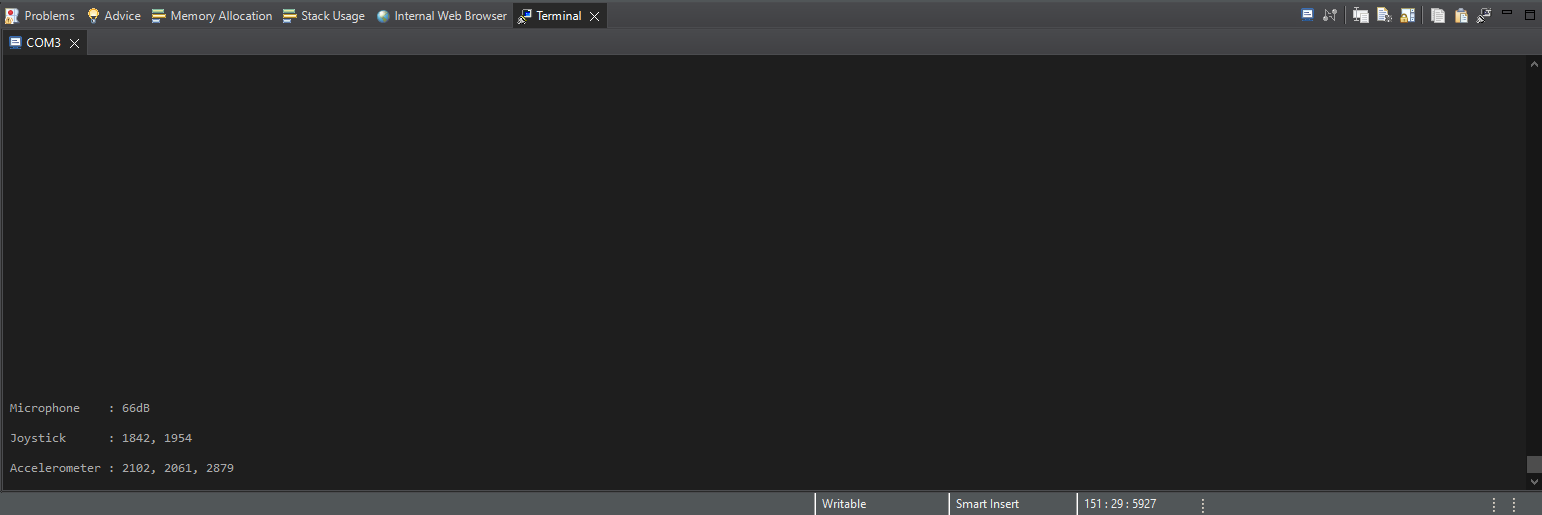
\includegraphics[width=\columnwidth]{images/assignment_3_output.png}
    \caption{Assignment 3 output serial terminal.}
    \label{fig:output}
\end{figure}

\begin{figure}[h]
    \centering
    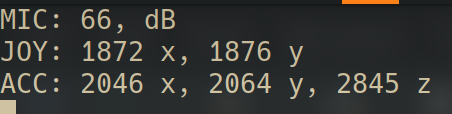
\includegraphics[width=\columnwidth]{images/4.3out.png}
    \caption{Assignment 3 output minicom terminal.}
    \label{fig:output_terminal}
\end{figure}
%\section{Discussion}
\label{section:disc}

%\section{Conclusion}
%\section*{Acknowledgment}
The authors would like to thank ... for his/her/their help and support during the process of writing this paper. 
% Select the IEEEtran style
%\bibliographystyle{IEEEtran}
% Include bibliography file
%\bibliography{IEEEabrv,references,DVA454}
\end{document}